\begin{figure}
  \centering
  \subfigure[SFI]{
    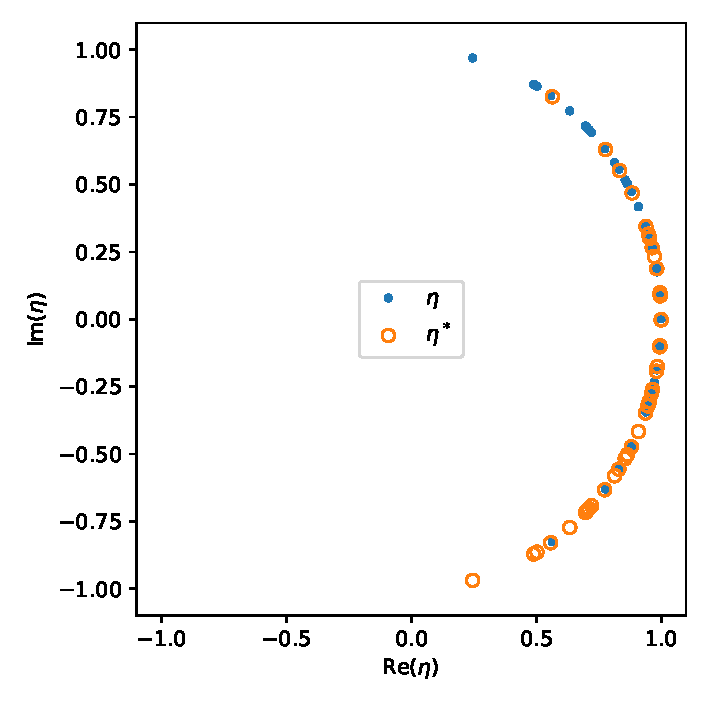
\includegraphics[width=0.44\textwidth]{../Plots/qmbs_sfim_N=06_tduration=0.5_Vrr=100_Omega=1.pdf}
  }
  \subfigure[PXP]{
    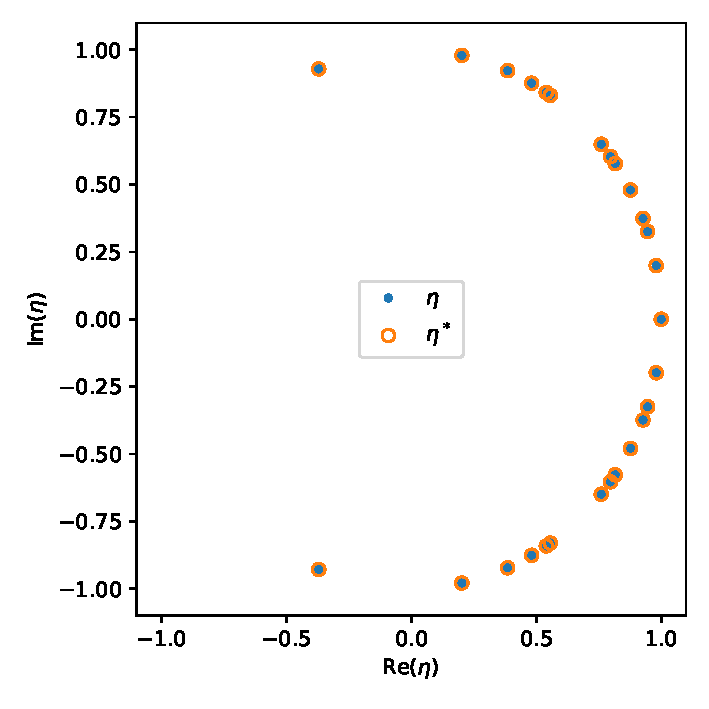
\includegraphics[width=0.44\textwidth]{../Plots/qmbs_pxp_N=06_tduration=0.5_Omega=1.pdf}
  }
  \caption{Eigenvalues $\eta$ (filled) and their complex conjugates
    $\eta^*$ (open) of the propagator, plotted in the complex plane for
    $N=6$, $\Omega t=0.5$. (a)~SFI with $V_{rr}=100\Omega$: the
    conjugates are reflections about the real axis, shown as a guide to
    the eye. (b)~PXP: the particle-hole symmetry
    $\Gamma = \prod_{l} Z_{l}$ of the PXP model at $\Delta = 0$ makes
    $\eta^*$ the eigenvalue of the partner state at energy $-E$.}
\end{figure}

\begin{figure}
  \centering
  \subfigure[SFI]{
    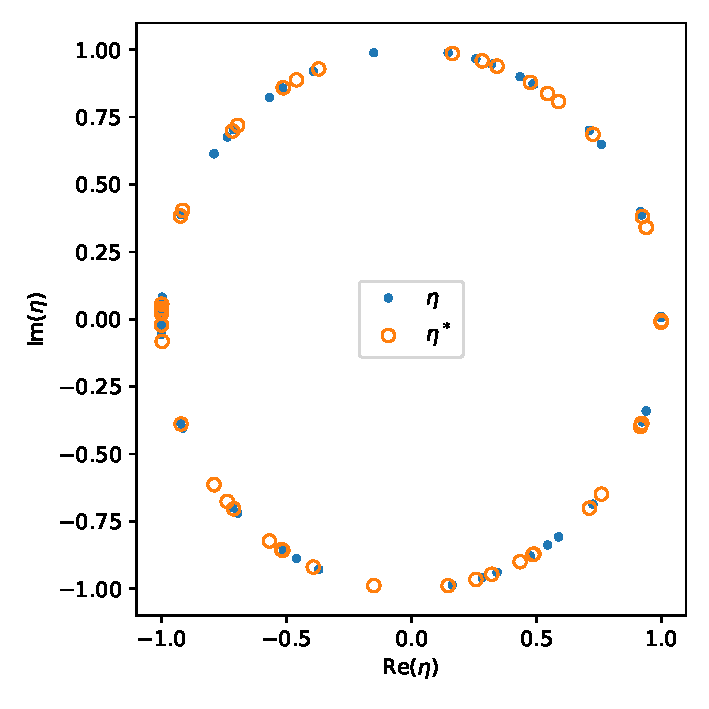
\includegraphics[width=0.44\textwidth]{../Plots/qmbs_sfim_N=06_tduration=2_Vrr=100_Omega=1.pdf}
  }
  \subfigure[PXP]{
    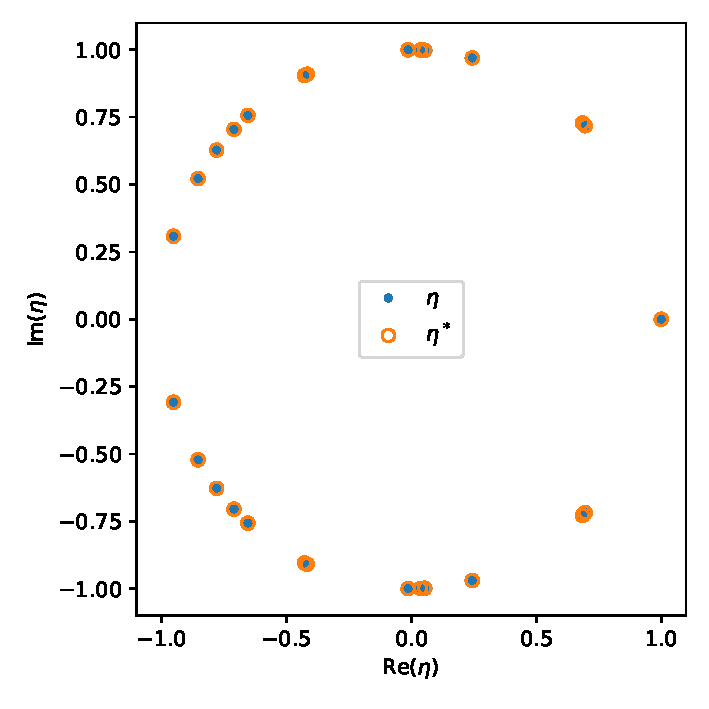
\includegraphics[width=0.44\textwidth]{../Plots/qmbs_pxp_N=06_tduration=2_Omega=1.pdf}
  }
  \caption{Eigenvalues $\eta$ (filled) and their complex conjugates
    $\eta^*$ (open) of the propagator, plotted in the complex plane for
    $N=6$, $\Omega t=2$. (a)~SFI with $V_{rr}=100\Omega$: the
    conjugates are reflections about the real axis, shown as a guide to
    the eye. (b)~PXP: the particle-hole symmetry
    $\Gamma = \prod_{l} Z_{l}$ of the PXP model at $\Delta = 0$ makes
    $\eta^*$ the eigenvalue of the partner state at energy $-E$.}
\end{figure}


\begin{figure}
  \centering
  \subfigure[SFI]{
    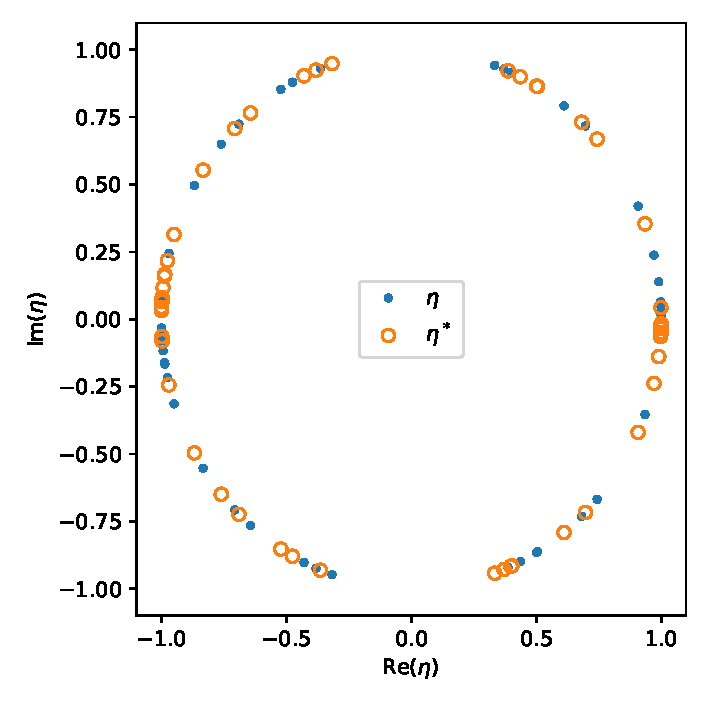
\includegraphics[width=0.44\textwidth]{../Plots/qmbs_sfim_N=06_tduration=6_Vrr=100_Omega=1.pdf}
  }
  \subfigure[PXP]{
    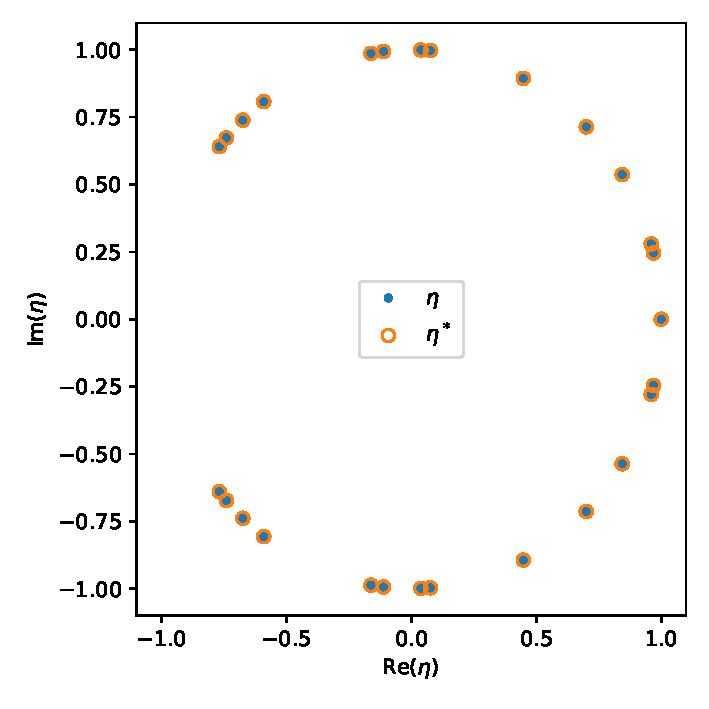
\includegraphics[width=0.44\textwidth]{../Plots/qmbs_pxp_N=06_tduration=6_Omega=1.pdf}
  }
  \caption{Eigenvalues $\eta$ (filled) and their complex conjugates
    $\eta^*$ (open) of the propagator, plotted in the complex plane for
    $N=6$, $\Omega t=6$. (a)~SFI with $V_{rr}=100\Omega$: the
    conjugates are reflections about the real axis, shown as a guide to
    the eye. (b)~PXP: the particle-hole symmetry
    $\Gamma = \prod_{l} Z_{l}$ of the PXP model at $\Delta = 0$ makes
    $\eta^*$ the eigenvalue of the partner state at energy $-E$.}
\end{figure}


\begin{figure}
  \centering
  \subfigure[SFI]{
    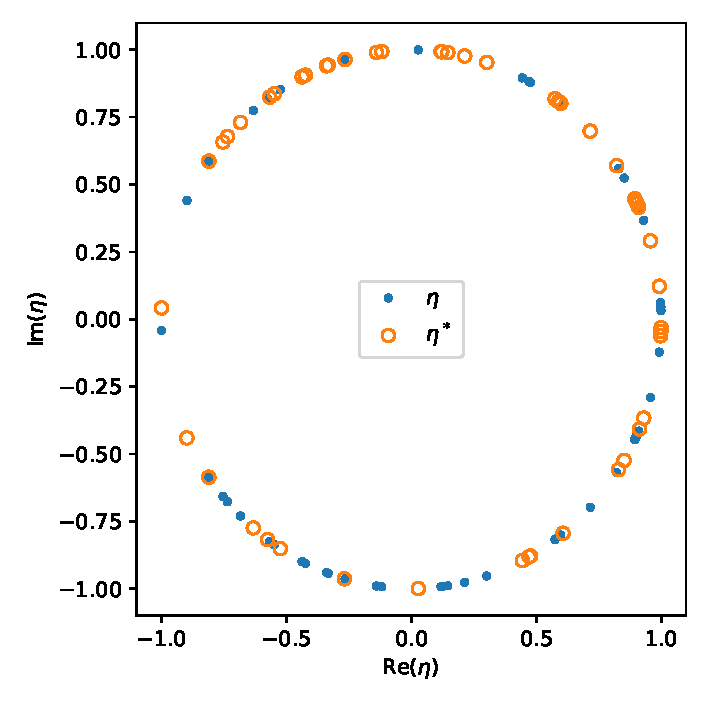
\includegraphics[width=0.44\textwidth]{../Plots/qmbs_sfim_N=06_tduration=11_Vrr=100_Omega=1.pdf}
  }
  \subfigure[PXP]{
    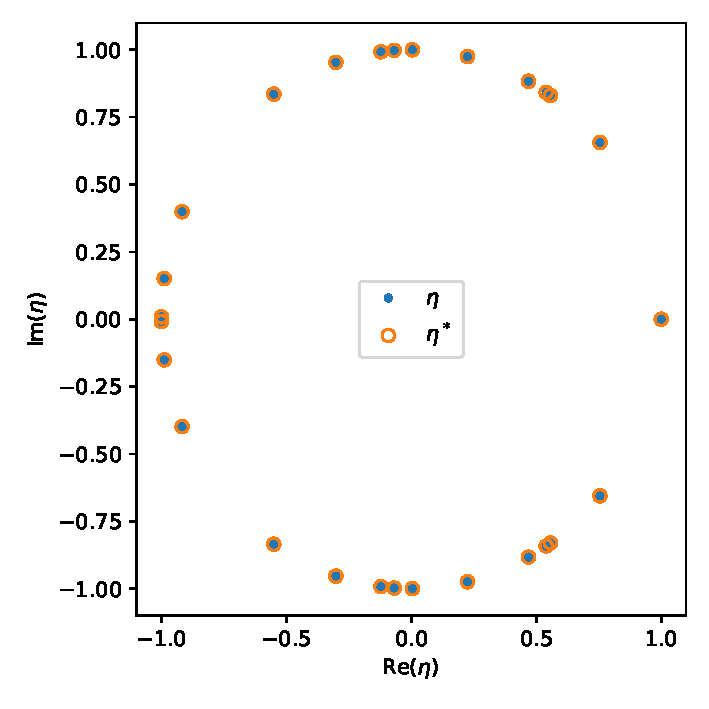
\includegraphics[width=0.44\textwidth]{../Plots/qmbs_pxp_N=06_tduration=11_Omega=1.pdf}
  }
  \caption{Eigenvalues $\eta$ (filled) and their complex conjugates
    $\eta^*$ (open) of the propagator, plotted in the complex plane for
    $N=6$, $\Omega t=11$. (a)~SFI with $V_{rr}=100\Omega$: the
    conjugates are reflections about the real axis, shown as a guide to
    the eye. (b)~PXP: the particle-hole symmetry
    $\Gamma = \prod_{l} Z_{l}$ of the PXP model at $\Delta = 0$ makes
    $\eta^*$ the eigenvalue of the partner state at energy $-E$.}
\end{figure}

%%%%%%%%%%%%%%%%

\begin{figure}
  \centering
  \subfigure[SFI]{
    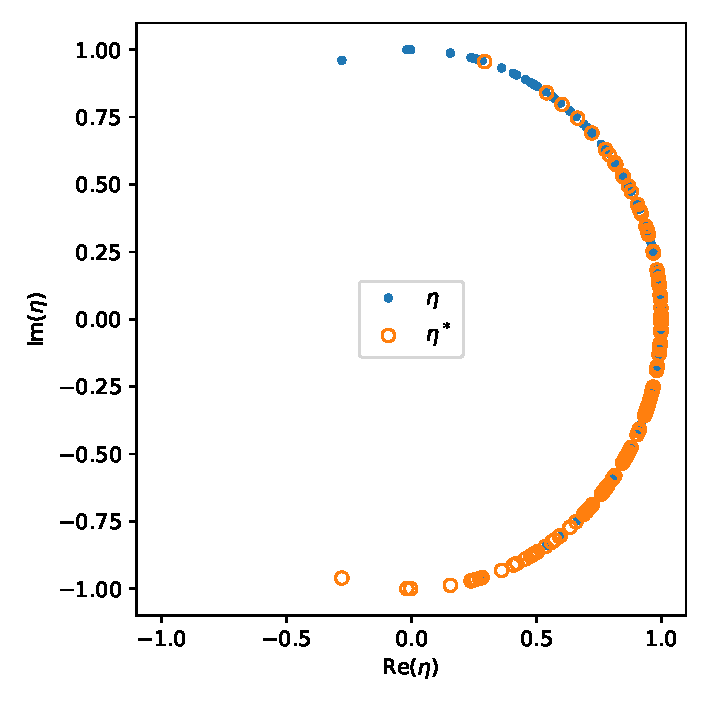
\includegraphics[width=0.44\textwidth]{../Plots/qmbs_sfim_N=08_tduration=0.5_Vrr=100_Omega=1.pdf}
  }
  \subfigure[PXP]{
    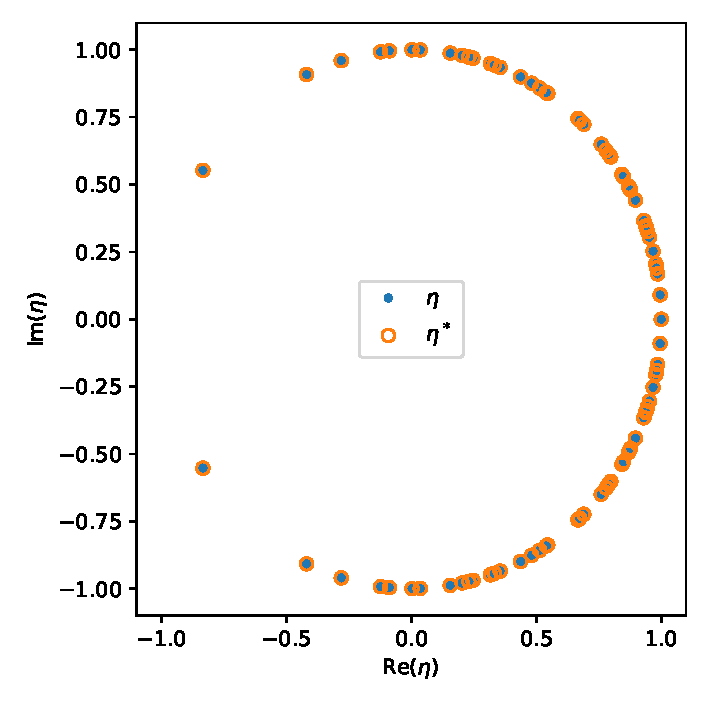
\includegraphics[width=0.44\textwidth]{../Plots/qmbs_pxp_N=08_tduration=0.5_Omega=1.pdf}
  }
  \caption{Eigenvalues $\eta$ (filled) and their complex conjugates
    $\eta^*$ (open) of the propagator, plotted in the complex plane for
    $N=8$, $\Omega t=0.5$. (a)~SFI with $V_{rr}=100\Omega$: the
    conjugates are reflections about the real axis, shown as a guide to
    the eye. (b)~PXP: the particle-hole symmetry
    $\Gamma = \prod_{l} Z_{l}$ of the PXP model at $\Delta = 0$ makes
    $\eta^*$ the eigenvalue of the partner state at energy $-E$.}
\end{figure}

\begin{figure}
  \centering
  \subfigure[SFI]{
    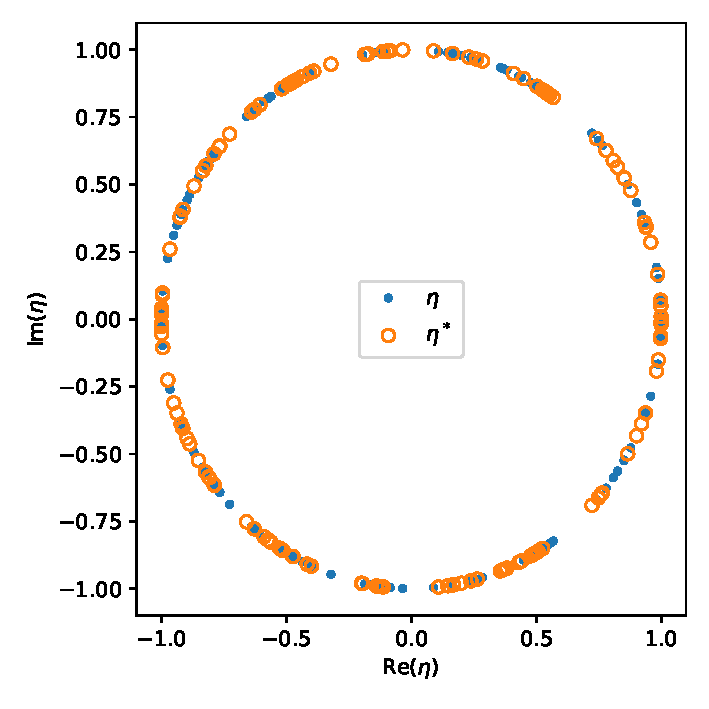
\includegraphics[width=0.44\textwidth]{../Plots/qmbs_sfim_N=08_tduration=2_Vrr=100_Omega=1.pdf}
  }
  \subfigure[PXP]{
    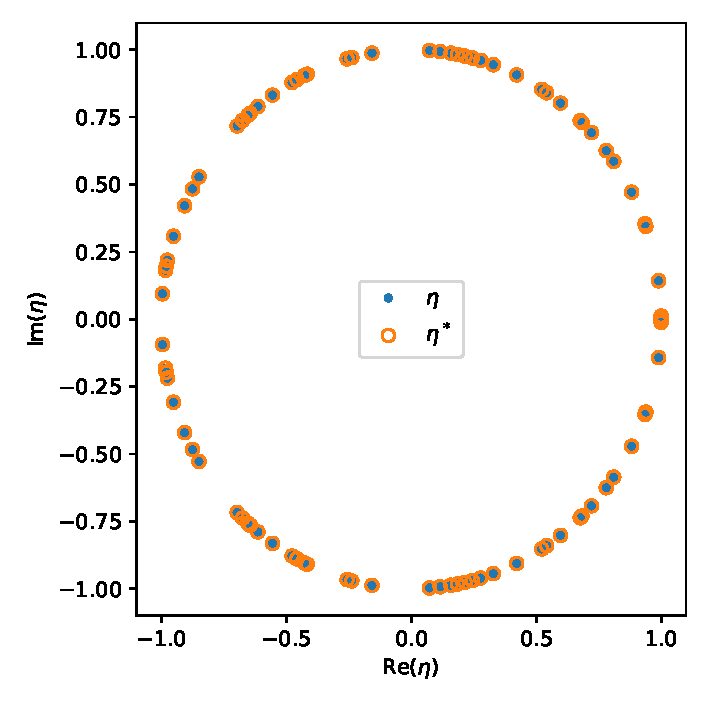
\includegraphics[width=0.44\textwidth]{../Plots/qmbs_pxp_N=08_tduration=2_Omega=1.pdf}
  }
  \caption{Eigenvalues $\eta$ (filled) and their complex conjugates
    $\eta^*$ (open) of the propagator, plotted in the complex plane for
    $N=8$, $\Omega t=2$. (a)~SFI with $V_{rr}=100\Omega$: the
    conjugates are reflections about the real axis, shown as a guide to
    the eye. (b)~PXP: the particle-hole symmetry
    $\Gamma = \prod_{l} Z_{l}$ of the PXP model at $\Delta = 0$ makes
    $\eta^*$ the eigenvalue of the partner state at energy $-E$.}
\end{figure}


\begin{figure}
  \centering
  \subfigure[SFI]{
    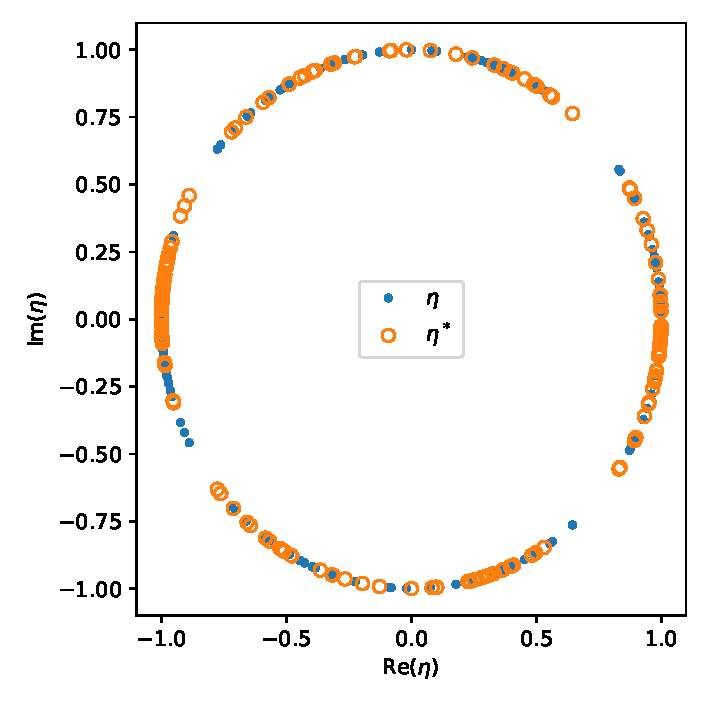
\includegraphics[width=0.44\textwidth]{../Plots/qmbs_sfim_N=08_tduration=6_Vrr=100_Omega=1.pdf}
  }
  \subfigure[PXP]{
    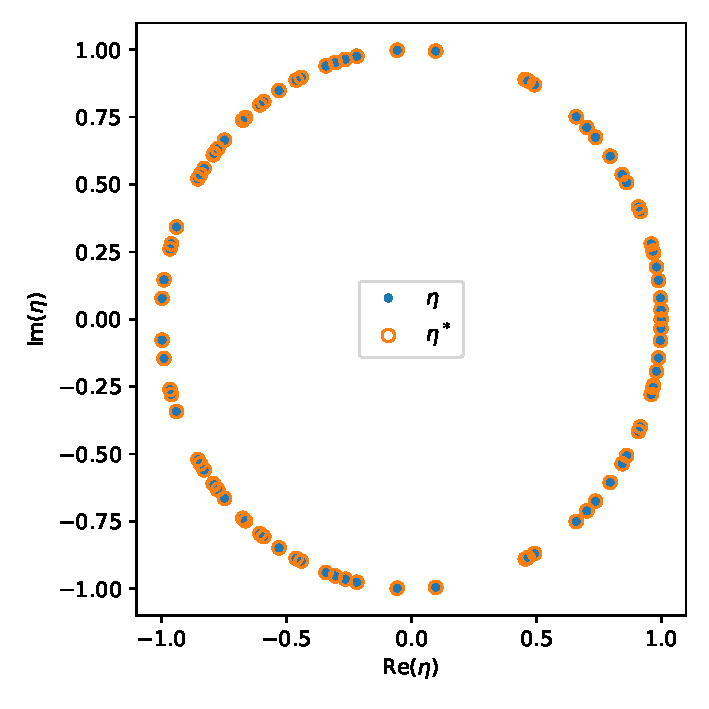
\includegraphics[width=0.44\textwidth]{../Plots/qmbs_pxp_N=08_tduration=6_Omega=1.pdf}
  }
  \caption{Eigenvalues $\eta$ (filled) and their complex conjugates
    $\eta^*$ (open) of the propagator, plotted in the complex plane for
    $N=8$, $\Omega t=6$. (a)~SFI with $V_{rr}=100\Omega$: the
    conjugates are reflections about the real axis, shown as a guide to
    the eye. (b)~PXP: the particle-hole symmetry
    $\Gamma = \prod_{l} Z_{l}$ of the PXP model at $\Delta = 0$ makes
    $\eta^*$ the eigenvalue of the partner state at energy $-E$.}
\end{figure}


\begin{figure}
  \centering
  \subfigure[SFI]{
    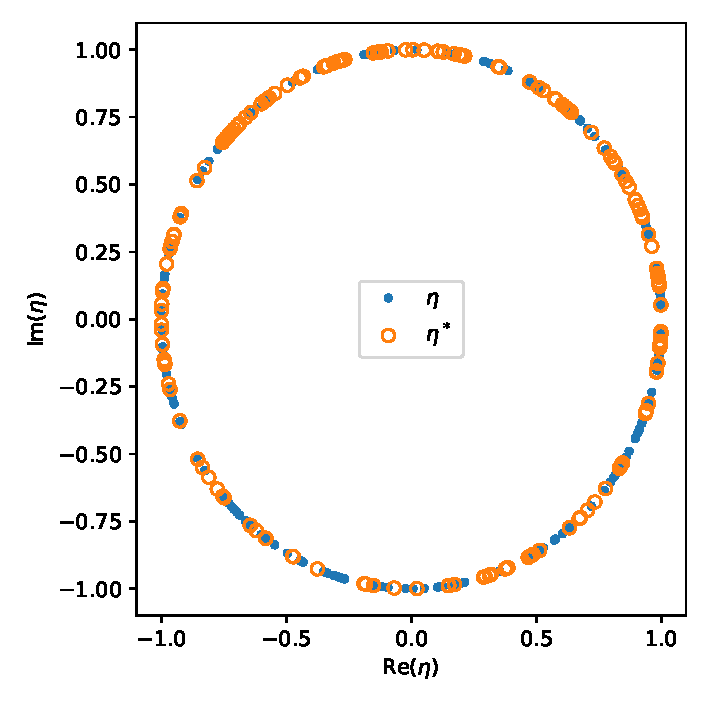
\includegraphics[width=0.44\textwidth]{../Plots/qmbs_sfim_N=08_tduration=11_Vrr=100_Omega=1.pdf}
  }
  \subfigure[PXP]{
    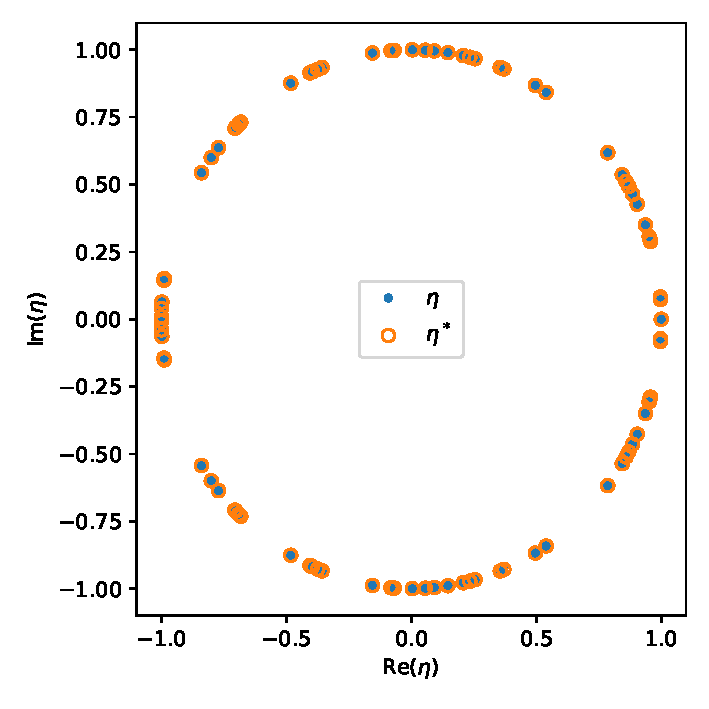
\includegraphics[width=0.44\textwidth]{../Plots/qmbs_pxp_N=08_tduration=11_Omega=1.pdf}
  }
  \caption{Eigenvalues $\eta$ (filled) and their complex conjugates
    $\eta^*$ (open) of the propagator, plotted in the complex plane for
    $N=8$, $\Omega t=11$. (a)~SFI with $V_{rr}=100\Omega$: the
    conjugates are reflections about the real axis, shown as a guide to
    the eye. (b)~PXP: the particle-hole symmetry
    $\Gamma = \prod_{l} Z_{l}$ of the PXP model at $\Delta = 0$ makes
    $\eta^*$ the eigenvalue of the partner state at energy $-E$.}
\end{figure}

%%%%%%%%%%%%%%%

\begin{figure}
  \centering
  \subfigure[SFI]{
    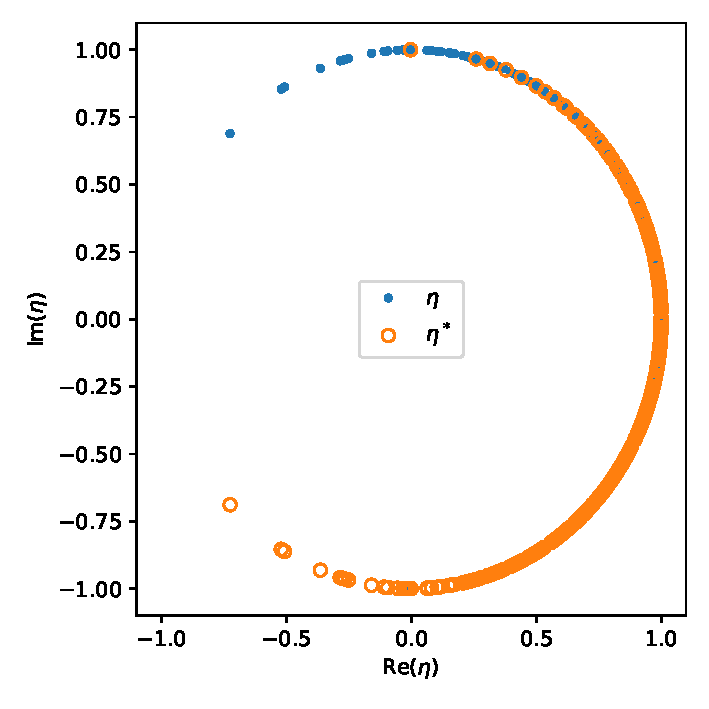
\includegraphics[width=0.44\textwidth]{../Plots/qmbs_sfim_N=10_tduration=0.5_Vrr=100_Omega=1.pdf}
  }
  \subfigure[PXP]{
    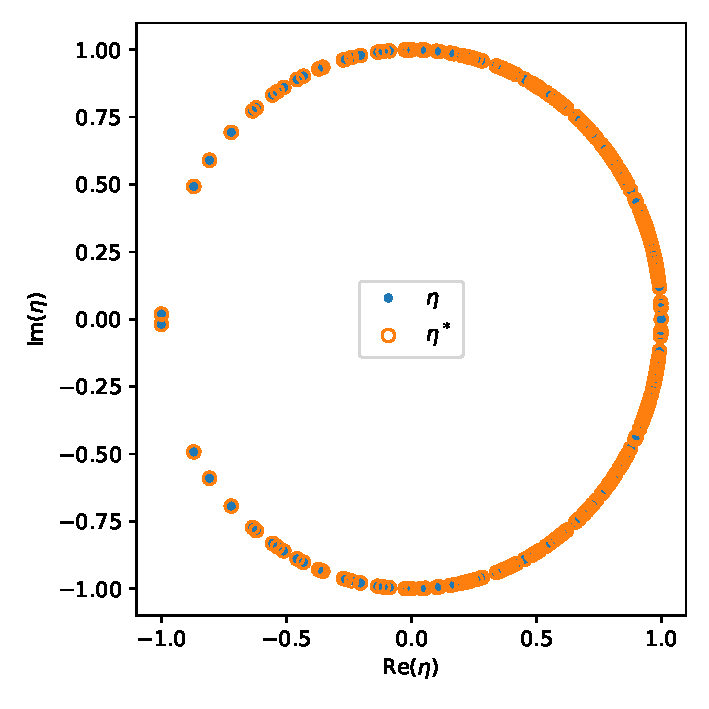
\includegraphics[width=0.44\textwidth]{../Plots/qmbs_pxp_N=10_tduration=0.5_Omega=1.pdf}
  }
  \caption{Eigenvalues $\eta$ (filled) and their complex conjugates
    $\eta^*$ (open) of the propagator, plotted in the complex plane for
    $N=10$, $\Omega t=0.5$. (a)~SFI with $V_{rr}=100\Omega$: the
    conjugates are reflections about the real axis, shown as a guide to
    the eye. (b)~PXP: the particle-hole symmetry
    $\Gamma = \prod_{l} Z_{l}$ of the PXP model at $\Delta = 0$ makes
    $\eta^*$ the eigenvalue of the partner state at energy $-E$.}
\end{figure}

\begin{figure}
  \centering
  \subfigure[SFI]{
    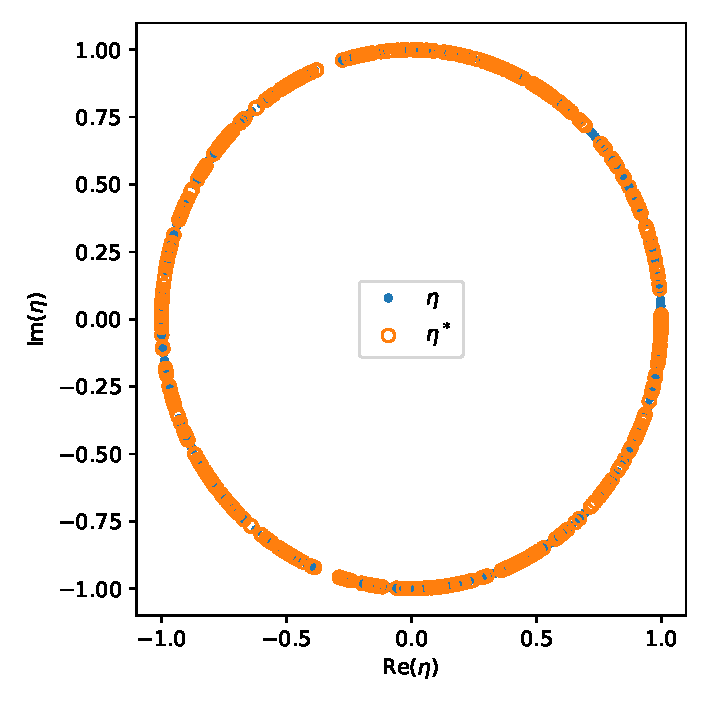
\includegraphics[width=0.44\textwidth]{../Plots/qmbs_sfim_N=10_tduration=2_Vrr=100_Omega=1.pdf}
  }
  \subfigure[PXP]{
    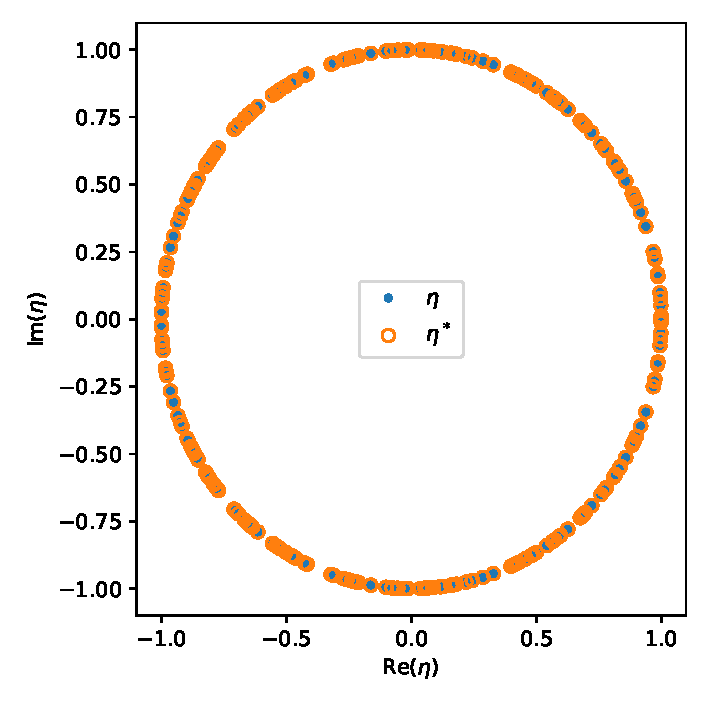
\includegraphics[width=0.44\textwidth]{../Plots/qmbs_pxp_N=10_tduration=2_Omega=1.pdf}
  }
  \caption{Eigenvalues $\eta$ (filled) and their complex conjugates
    $\eta^*$ (open) of the propagator, plotted in the complex plane for
    $N=10$, $\Omega t=2$. (a)~SFI with $V_{rr}=100\Omega$: the
    conjugates are reflections about the real axis, shown as a guide to
    the eye. (b)~PXP: the particle-hole symmetry
    $\Gamma = \prod_{l} Z_{l}$ of the PXP model at $\Delta = 0$ makes
    $\eta^*$ the eigenvalue of the partner state at energy $-E$.}
\end{figure}


\begin{figure}
  \centering
  \subfigure[SFI]{
    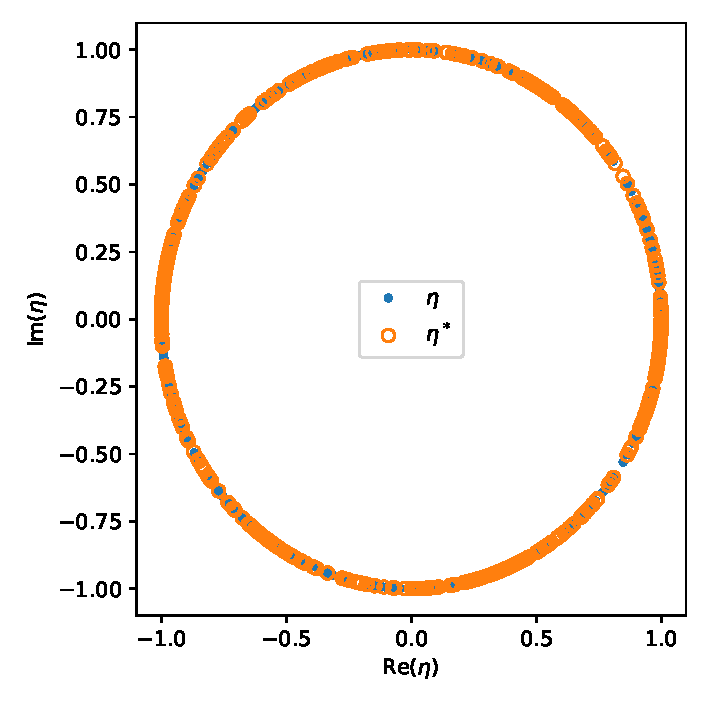
\includegraphics[width=0.44\textwidth]{../Plots/qmbs_sfim_N=10_tduration=6_Vrr=100_Omega=1.pdf}
  }
  \subfigure[PXP]{
    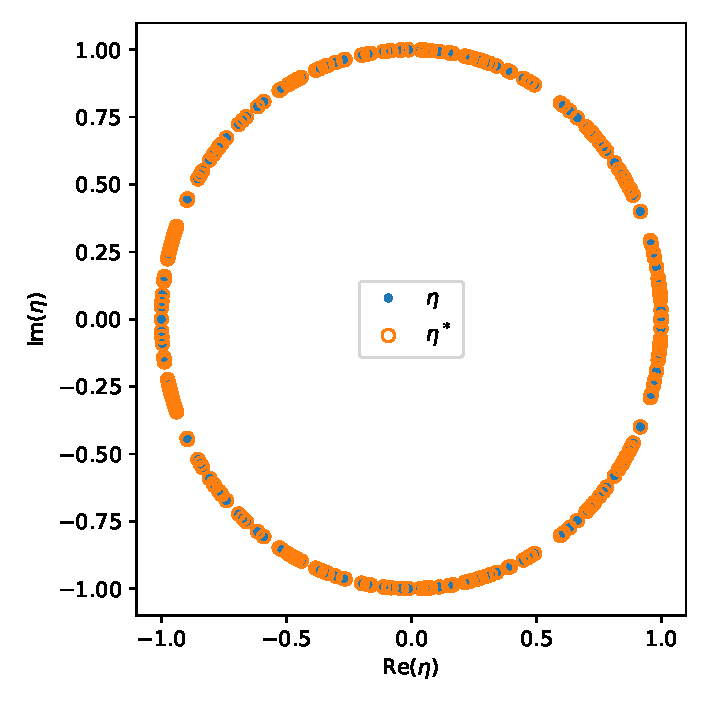
\includegraphics[width=0.44\textwidth]{../Plots/qmbs_pxp_N=10_tduration=6_Omega=1.pdf}
  }
  \caption{Eigenvalues $\eta$ (filled) and their complex conjugates
    $\eta^*$ (open) of the propagator, plotted in the complex plane for
    $N=10$, $\Omega t=6$. (a)~SFI with $V_{rr}=100\Omega$: the
    conjugates are reflections about the real axis, shown as a guide to
    the eye. (b)~PXP: the particle-hole symmetry
    $\Gamma = \prod_{l} Z_{l}$ of the PXP model at $\Delta = 0$ makes
    $\eta^*$ the eigenvalue of the partner state at energy $-E$.}
\end{figure}


\begin{figure}
  \centering
  \subfigure[SFI]{
    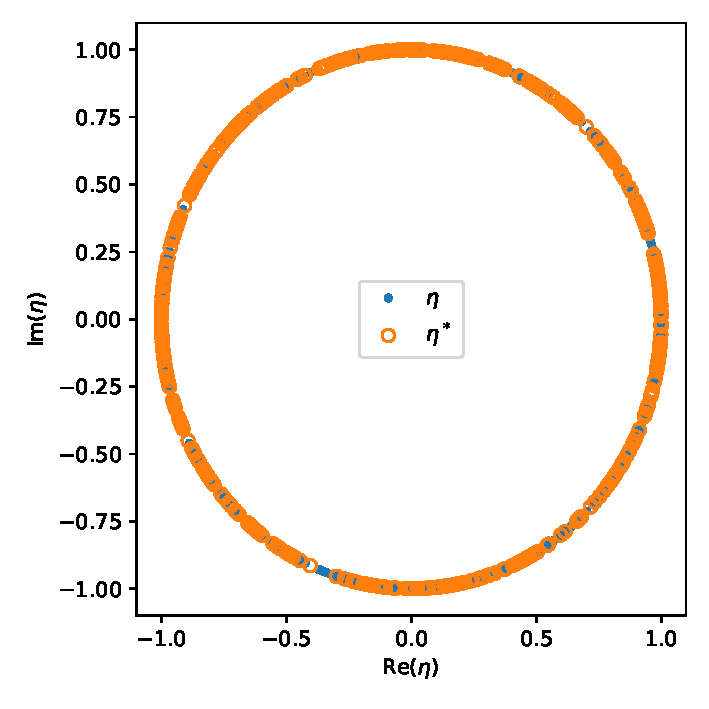
\includegraphics[width=0.44\textwidth]{../Plots/qmbs_sfim_N=10_tduration=11_Vrr=100_Omega=1.pdf}
  }
  \subfigure[PXP]{
    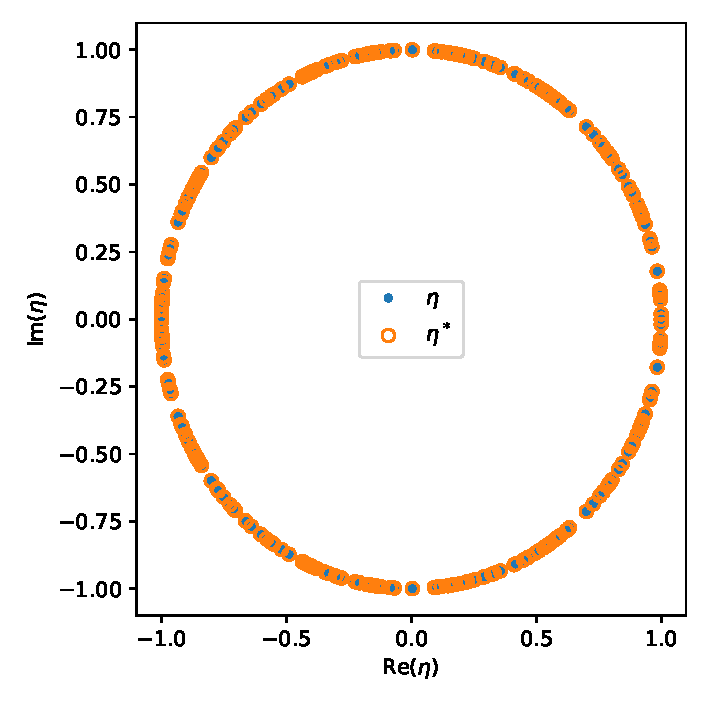
\includegraphics[width=0.44\textwidth]{../Plots/qmbs_pxp_N=10_tduration=11_Omega=1.pdf}
  }
  \caption{Eigenvalues $\eta$ (filled) and their complex conjugates
    $\eta^*$ (open) of the propagator, plotted in the complex plane for
    $N=10$, $\Omega t=11$. (a)~SFI with $V_{rr}=100\Omega$: the
    conjugates are reflections about the real axis, shown as a guide to
    the eye. (b)~PXP: the particle-hole symmetry
    $\Gamma = \prod_{l} Z_{l}$ of the PXP model at $\Delta = 0$ makes
    $\eta^*$ the eigenvalue of the partner state at energy $-E$.}
\end{figure}
